\section{Results}\label{sec:results}

Figure~\ref{fig:forest} shows the HOTA difference between each host with
\scl{} and the host alone for every tested cell. The next subsections give
the baseline comparison for each part of the evaluation, in the order of the
three expectations of Sect.~\ref{sec:setup}: well-matched trackers, trackers
that do not fit their detector, and systems not seen during design.

\begin{figure}[t]
\centering
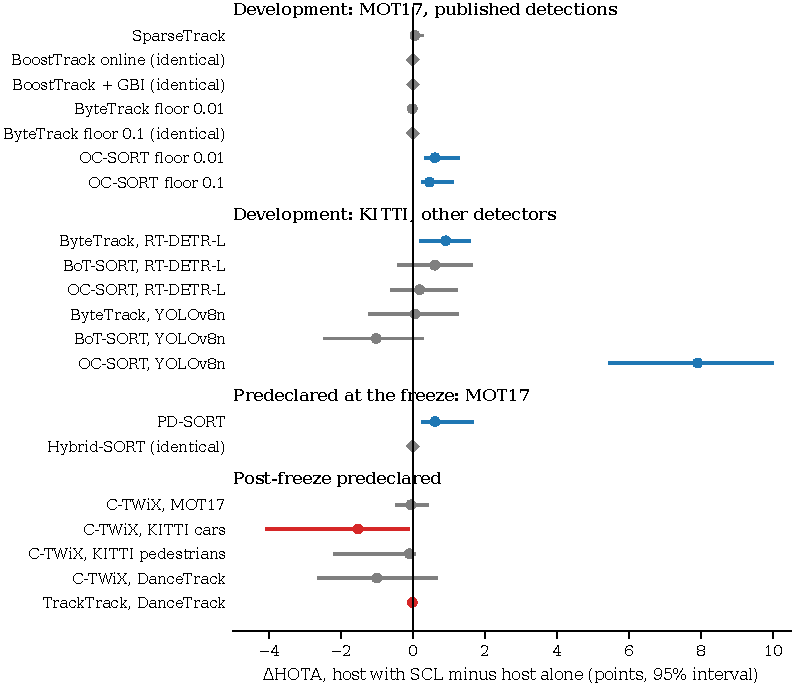
\includegraphics[width=0.82\textwidth]{figures/fig3_forest.pdf}
\caption{Difference in HOTA (host with \scl{} minus host alone) with
95\% paired-bootstrap interval for every tested cell. Blue: interval above
zero; red: interval below zero; gray: interval contains zero. Diamonds mark
identical output.}
\label{fig:forest}
\end{figure}

\subsection{Results across trackers}\label{sec:tracker}
Table~\ref{tab:mot17} compares the development trackers with their hosts on
MOT17. The two-stage trackers with well-matched detections stayed at the
accuracy of their hosts. BoostTrack, online and with interpolation, and
ByteTrack at floor 0.1 gave identical output. ByteTrack at floor 0.01
changed by $-0.014$ HOTA and SparseTrack by $+0.055$. This is the
self-limiting behavior of the clean mode (Sect.~\ref{sec:regimes}), which
the earlier design did not have (Table~\ref{tab:prior}).

The single-stage OC-SORT improved at both emission floors. Its HOTA rose by
0.61 points ($[+0.36,+1.24]$) at floor 0.01 and by 0.46 points
($[+0.27,+1.09]$) at floor 0.1, and its MOTA by 1.27 and 1.26 points. HOTA
was higher on 7 of 7 sequences in both settings (Fig.~\ref{fig:perseq}). The
gain comes from the continuation rescue. OC-SORT drops every detection
below its single threshold, and the layer passes it the foreground candidates
that continue a track that would otherwise stay unmatched.

\begin{table}[t]
\caption{Baseline comparison of the development trackers on MOT17 val-half
(published YOLOX-X detections). Paper: number reported by the tracker's
authors. Host: published tracker alone (our reproduction). $\Delta$: host with
\scl{} minus host, with 95\% paired-bootstrap interval (10,000
resamples, seed 42); bold intervals exclude zero. The floor is the lowest
detector score emitted.}
\label{tab:mot17}
\centering\footnotesize
\setlength{\tabcolsep}{4pt}
\begin{tabular}{@{}lrrl@{}}
\toprule
Metric & Paper & Host & $\Delta$ [95\% CI]\\
\midrule
\multicolumn{4}{@{}l}{\textit{SparseTrack} \cite{liu2025sparsetrack}}\\
\quad HOTA & 69.2 & 68.88 & $+0.06$ [$-0.01$, $+0.25$]\\
\quad MOTA & 76.8 & 77.85 & $+0.08$ [$-0.03$, $+0.30$]\\
\quad IDF1 & 81.4 & 81.97 & $+0.16$ [$-0.02$, $+0.70$]\\
\multicolumn{4}{@{}l}{\textit{BoostTrack, online} \cite{stanojevic2024boosttrack}}\\
\quad HOTA & 68.37 & 68.49 & 0 (identical)\\
\quad MOTA & 75.56 & 75.50 & 0 (identical)\\
\quad IDF1 & 81.35 & 81.41 & 0 (identical)\\
\multicolumn{4}{@{}l}{\textit{BoostTrack, + GBI} \cite{stanojevic2024boosttrack}}\\
\quad HOTA & 71.33 & 71.72 & 0 (identical)\\
\quad MOTA & 80.55 & 81.03 & 0 (identical)\\
\quad IDF1 & 83.84 & 84.16 & 0 (identical)\\
\multicolumn{4}{@{}l}{\textit{ByteTrack, floor 0.01} \cite{zhang2022bytetrack}}\\
\quad HOTA & -- & 67.70 & $-0.014$ [$-0.058$, $+0.009$]\\
\quad MOTA & 76.6 & 77.60 & $+0.06$ [$-0.15$, $+0.34$]\\
\quad IDF1 & 79.3 & 79.47 & $-0.031$ [$-0.135$, $+0.035$]\\
\multicolumn{4}{@{}l}{\textit{ByteTrack, floor 0.1} \cite{zhang2022bytetrack}}\\
\quad HOTA & -- & 67.70 & 0 (identical)\\
\quad MOTA & 76.6 & 77.60 & 0 (identical)\\
\quad IDF1 & 79.3 & 79.47 & 0 (identical)\\
\multicolumn{4}{@{}l}{\textit{OC-SORT, floor 0.01} \cite{cao2023ocsort}}\\
\quad HOTA & 66.5 & 66.43 & {\boldmath $+0.61$ [$+0.36$, $+1.24$]}\\
\quad MOTA & 74.9 & 74.67 & {\boldmath $+1.27$ [$+0.17$, $+3.01$]}\\
\quad IDF1 & 77.7 & 78.05 & $+0.66$ [$-0.25$, $+1.60$]\\
\multicolumn{4}{@{}l}{\textit{OC-SORT, floor 0.1} \cite{cao2023ocsort}}\\
\quad HOTA & 66.5 & 66.44 & {\boldmath $+0.46$ [$+0.27$, $+1.09$]}\\
\quad MOTA & 74.9 & 74.67 & {\boldmath $+1.26$ [$+0.37$, $+3.34$]}\\
\quad IDF1 & 77.7 & 78.05 & {\boldmath $+0.287$ [$+0.003$, $+0.838$]}\\
\bottomrule
\end{tabular}
\end{table}


\begin{figure}[t]
\centering
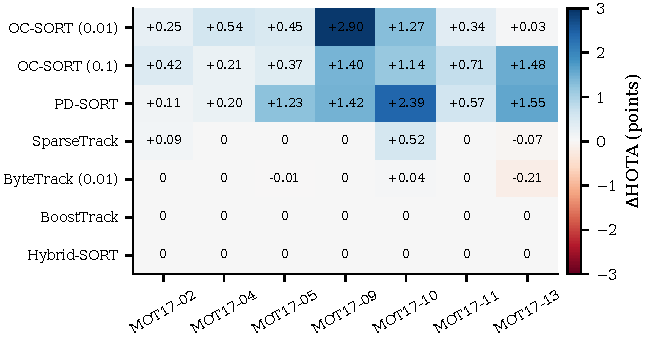
\includegraphics[width=0.75\textwidth]{figures/fig4_per_sequence.pdf}
\caption{Per-sequence HOTA differences (host with \scl{} minus host
alone) on MOT17 val-half for the development trackers and the external
trackers declared at the freeze.}
\label{fig:perseq}
\end{figure}

\subsection{Results with other detectors}\label{sec:detector}
Table~\ref{tab:kitti} reports all six KITTI cells: three trackers with each of
the two other detectors. With the noisy RT-DETR-L detector, the two-stage
trackers gained in MOTA and IDF1. ByteTrack gained 5.98 MOTA points
($[+1.16,+9.94]$), 3.87 IDF1 points, and 0.91 HOTA points
($[+0.22,+1.55]$). BoT-SORT gained 7.86 MOTA points ($[+2.21,+13.44]$) and
3.10 IDF1 points. OC-SORT with RT-DETR-L changed by less than 0.6 points in
every metric, with all intervals including zero. With YOLOv8n, the
single-stage OC-SORT gained 7.91 HOTA points ($[+5.47,+9.98]$), 9.40 MOTA
points, and 9.60 IDF1 points.

The two two-stage trackers with YOLOv8n are the regression case of the
development data. Their HOTA changed by $+0.06$ (ByteTrack) and $-1.02$
(BoT-SORT), both with intervals including zero, but their MOTA fell by 1.87
($[-6.25,+0.03]$) and 2.43 points ($[-7.43,-0.14]$), while identity switches
fell by 271 and 227, about half of the hosts' own counts. YOLOv8n gives many
correct detections with low scores, so the layer classified these streams as
noisy and allowed new tracks only from the confident group. This restriction
cost MOTA while it reduced identity switches. The regression was known when
the configuration was frozen.

\begin{table}[t]
\caption{Baseline comparison under a detector change on KITTI tracking
training (official HOTA, car and pedestrian averaged), all six cells. Host:
published tracker alone with the same detections. $\Delta$: host with \scl{}
minus host, with 95\% paired-bootstrap interval; bold intervals exclude zero.
BoT-SORT uses 20 of the 21 sequences in both arms: on sequence 0020, the
BoT-SORT Kalman update failed with a numerical (Cholesky) error when it
received the layer's output, while the host alone ran normally. This failure
case is excluded from both arms.}
\label{tab:kitti}
\centering\footnotesize
\setlength{\tabcolsep}{4pt}
\begin{tabular}{@{}lrlrl@{}}
\toprule
 & \multicolumn{2}{c}{RT-DETR-L} & \multicolumn{2}{c}{YOLOv8n}\\
\cmidrule(lr){2-3}\cmidrule(l){4-5}
Metric & Host & $\Delta$ [95\% CI] & Host & $\Delta$ [95\% CI]\\
\midrule
\multicolumn{5}{@{}l}{\textit{ByteTrack} \cite{zhang2022bytetrack}\textit{, library setting}}\\
\quad HOTA & 50.73 & {\boldmath $+0.91$ [$+0.22$, $+1.55$]} & 45.31 & $+0.06$ [$-1.19$, $+1.24$]\\
\quad MOTA & 47.27 & {\boldmath $+5.98$ [$+1.16$, $+9.94$]} & 46.54 & $-1.87$ [$-6.25$, $+0.03$]\\
\quad IDF1 & 64.98 & {\boldmath $+3.87$ [$+1.67$, $+5.06$]} & 60.92 & $+1.49$ [$-0.36$, $+3.27$]\\
\multicolumn{5}{@{}l}{\textit{BoT-SORT} \cite{aharon2022botsort}\textit{, library setting (20 sequences)}}\\
\quad HOTA & 53.91 & $+0.61$ [$-0.39$, $+1.61$] & 49.21 & $-1.02$ [$-2.43$, $+0.25$]\\
\quad MOTA & 48.25 & {\boldmath $+7.86$ [$+2.21$, $+13.44$]} & 49.89 & {\boldmath $-2.43$ [$-7.43$, $-0.14$]}\\
\quad IDF1 & 67.74 & {\boldmath $+3.10$ [$+1.00$, $+4.57$]} & 64.41 & $+0.35$ [$-2.10$, $+2.27$]\\
\multicolumn{5}{@{}l}{\textit{OC-SORT} \cite{cao2023ocsort}}\\
\quad HOTA & 52.64 & $+0.19$ [$-0.57$, $+1.19$] & 36.27 & {\boldmath $+7.91$ [$+5.47$, $+9.98$]}\\
\quad MOTA & 57.59 & $-0.57$ [$-4.36$, $+1.40$] & 33.99 & {\boldmath $+9.40$ [$+1.10$, $+12.30$]}\\
\quad IDF1 & 69.87 & $+0.04$ [$-1.31$, $+1.78$] & 50.46 & {\boldmath $+9.60$ [$+5.61$, $+12.16$]}\\
\bottomrule
\end{tabular}
\end{table}


\subsection{Results under shifted detector scores}\label{sec:shift}
Table~\ref{tab:shift} and Fig.~\ref{fig:shift} show the trackers under the
four score transforms. Halving the scores reduced ByteTrack (official setting)
and OC-SORT to 0 HOTA, because no detection reached their thresholds. With the
layer they reached 66.17 and 66.72. Cubing reduced them to 60.92 and 58.34,
and the layer restored them to 65.81 and 66.60. BoostTrack rose from 61.33 to
64.84 under cubing. With temperature $T=2$, the layer raised ByteTrack and
OC-SORT by 1.11 and 1.24 points. The library setting of ByteTrack, whose low
thresholds already accept the changed scores, stayed within 0.14 points in all
four transforms. Over the 14 conditions, the layer raised HOTA significantly
in 7 and lowered it significantly in none.

\begin{table}[t]
\caption{Baseline comparison under shifted detector scores on MOT17 val-half
(HOTA). The detector scores are transformed before the tracker, whose
published thresholds stay fixed; $T$ is a logit temperature, $\sigma(z/T)$.
Host: published tracker alone. $\Delta$: with \scl{} minus host,
with 95\% paired-bootstrap interval (10,000 resamples, seed 42). Bold
intervals exclude zero. Emission floor 0.01 (BoostTrack 0.1).}
\label{tab:shift}
\centering\footnotesize
\setlength{\tabcolsep}{4pt}
\begin{tabular}{@{}lrrl@{}}
\toprule
Transform & Host & + \scl{} & $\Delta$HOTA\\
\midrule
\multicolumn{4}{@{}l}{\textit{ByteTrack, official setting} \cite{zhang2022bytetrack}}\\
\quad $s^3$ & 60.92 & 65.81 & {\boldmath $+4.89$ [$+2.60$, $+13.69$]}\\
\quad $0.5\,s$ & 0.00 & 66.17 & {\boldmath $+66.17$ [$+49.32$, $+75.40$]}\\
\quad $T=2$ & 65.84 & 66.95 & {\boldmath $+1.11$ [$+0.35$, $+3.87$]}\\
\quad $T=0.5$ & 67.30 & 67.29 & $-0.009$ [$-0.051$, $+0.005$]\\
\multicolumn{4}{@{}l}{\textit{ByteTrack, library setting} \cite{zhang2022bytetrack}}\\
\quad $s^3$ & 66.31 & 66.31 & $-0.006$ [$-0.384$, $+0.383$]\\
\quad $0.5\,s$ & 66.61 & 66.48 & $-0.14$ [$-0.66$, $+0.14$]\\
\quad $T=2$ & 63.97 & 63.97 & 0 (identical)\\
\quad $T=0.5$ & 66.53 & 66.52 & $-0.006$ [$-0.029$, $+0.001$]\\
\multicolumn{4}{@{}l}{\textit{OC-SORT} \cite{cao2023ocsort}}\\
\quad $s^3$ & 58.34 & 66.60 & {\boldmath $+8.26$ [$+5.86$, $+16.81$]}\\
\quad $0.5\,s$ & 0.00 & 66.72 & {\boldmath $+66.72$ [$+50.32$, $+75.56$]}\\
\quad $T=2$ & 65.99 & 67.22 & {\boldmath $+1.24$ [$+0.52$, $+3.42$]}\\
\quad $T=0.5$ & 66.61 & 67.06 & $+0.45$ [$-0.01$, $+0.97$]\\
\multicolumn{4}{@{}l}{\textit{BoostTrack, online} \cite{stanojevic2024boosttrack}}\\
\quad $s^3$ & 61.33 & 64.84 & {\boldmath $+3.51$ [$+0.85$, $+13.28$]}\\
\quad $T=2$ & 67.59 & 67.59 & 0 (identical)\\
\bottomrule
\end{tabular}
\end{table}


\begin{figure}[t]
\centering
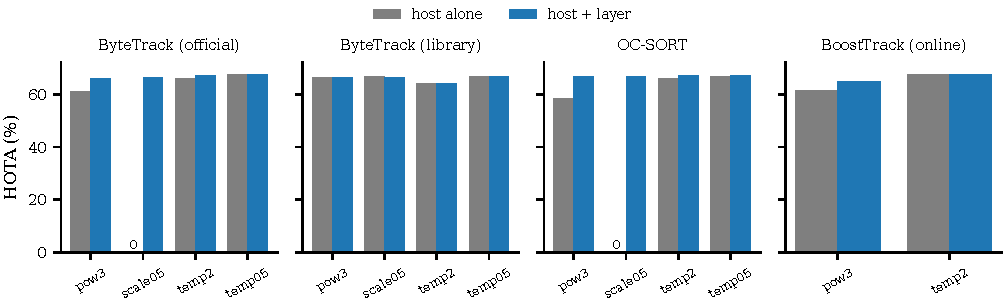
\includegraphics[width=\textwidth]{figures/fig5_calibration_shift.pdf}
\caption{Shifted detector scores on MOT17 val-half: HOTA of each published
tracker with its published thresholds, alone and with \scl{}, after
four monotone transforms of the detector scores (pow3: $s^3$; scale05:
$0.5\,s$; temp2 and temp05: $T=2$ and $T=0.5$).}
\label{fig:shift}
\end{figure}

\subsection{Results on external trackers}\label{sec:external}
Table~\ref{tab:external} gives every external system that passed its
reproduction. The external tests use new trackers on public benchmarks, each
with the detections that its authors released, so they test the transfer of
the frozen configuration to trackers, and with C-TWiX and TrackTrack also to
other detectors and datasets; they do not use new data.

\emph{Declared at the freeze.} PD-SORT \cite{wang2025pdsort} was reproduced
exactly as in the authors' released output. With \scl{}, its HOTA rose by 0.61
points ($[+0.27,+1.65]$), its MOTA by 1.13 points ($[+0.27,+3.03]$), and its
IDF1 by 0.82 points ($[+0.43,+1.94]$), with higher HOTA on 7 of 7 sequences
(Fig.~\ref{fig:perseq}). FN fell by 1,291, and FP rose by 681. PD-SORT is a
single-stage tracker, and its gain comes from the same step as for OC-SORT;
unlike OC-SORT, it was not seen during design. Hybrid-SORT
\cite{yang2024hybridsort}, a two-stage tracker, gave identical output, as
predicted before the run. Its reproduction was 0.40 HOTA below the authors'
number (CLOSE). The likely causes are the half-precision detections released
by the authors, whereas their reported number used full-precision inference,
and the software environment; the cause was documented but not isolated.

\emph{Declared after the freeze.} C-TWiX \cite{miah2025twix}, a single-stage
tracker that learns association from box coordinates, was reproduced on three
datasets: exactly on KITTI cars (89.27 against 89.3 HOTA), and within the
CLOSE class on KITTI pedestrians (70.77 against 71.4), MOT17 (77.55 against
77.8), and DanceTrack (59.62 against 60.4). It ran with the authors'
half-precision setting, but on a CPU instead of a GPU. On MOT17 the layer changed its HOTA
by $-0.05$ ($[-0.46,+0.40]$), on KITTI pedestrians by $-0.10$
($[-2.16,+0.03]$), and on DanceTrack by $-1.00$ ($[-2.62,+0.65]$). On KITTI
cars it lowered HOTA by 1.52 points ($[-4.05,-0.13]$), the only significant
external HOTA loss larger than 0.1 points. TrackTrack \cite{shim2025tracktrack}, a
two-stage tracker, was reproduced within 0.34 HOTA on DanceTrack (CLOSE, with
full-precision appearance features on a CPU). The layer changed its HOTA by
$-0.013$ ($[-0.032,-0.001]$): the interval excludes zero, but the effect is
negligible, and 21 of 25 sequences were tied. TOPICTrack failed its
reproduction and is excluded (Sect.~\ref{sec:setup}); the layer's effect on it
($-0.016$ HOTA, interval including zero) was recorded but is not analyzed.

The protocol also fixed predictions before these runs. For C-TWiX on MOT17 it
predicted no loss in HOTA; the measured $-0.05$ is a small loss with an
interval including zero, so the prediction did not hold. For KITTI and
DanceTrack it predicted a change of less than one HOTA point; this held for
KITTI pedestrians but not for KITTI cars ($-1.52$) or DanceTrack ($-1.00$).
For TOPICTrack, a change of at most 0.1 points was predicted and observed,
but this system is excluded. Section~\ref{sec:discussion} analyzes the
C-TWiX losses.

\begin{table*}[t]
\caption{Baseline comparison on the external systems, each run once with the frozen \scl{}.
Top: declared at the freeze (MOT17 val-half, authors' released detections). Bottom:
declared after the freeze under the registered protocol (authors' released detections;
TrackTrack after its post-processing, as in its paper). Ref.: HOTA reported by the
authors (for PD-SORT, their released output). Class: reproduction against Ref. (EXACT:
$|\Delta\mathrm{HOTA}|\le0.2$; CLOSE: $\le1.0$ with a documented, untuned cause).
Host: HOTA of the published tracker alone (our reproduction). $\Delta$: host with \scl{}
minus host, with the 95\% paired-bootstrap interval below it; bold intervals exclude zero.
W/T/L: sequences where HOTA rose, stayed within 0.01, or fell; ped.: pedestrians. TOPICTrack (FAILED
reproduction) is excluded.}
\label{tab:external}
\centering\footnotesize
\setlength{\tabcolsep}{2.5pt}
\renewcommand{\arraystretch}{1.15}
\begin{tabular}{@{}llccccc@{}}
\toprule
System (class) & Data & \twol{Ref.}{Host} & $\Delta$HOTA & $\Delta$MOTA & $\Delta$IDF1 & W/T/L\\
\midrule
\twol{PD-SORT \cite{wang2025pdsort}}{(EXACT)} & MOT17 & \twol{68.01}{68.01} & \cib{+0.61}{+0.27}{+1.65} & \cib{+1.13}{+0.27}{+3.03} & \cib{+0.82}{+0.43}{+1.94} & 7/0/0\\
\twol{Hybrid-SORT \cite{yang2024hybridsort}}{(CLOSE)} & MOT17 & \twol{67.1}{66.70} & \twol{0}{(identical)} & 0 & 0 & 0/7/0\\
\midrule
\twol{C-TWiX \cite{miah2025twix}}{(CLOSE)} & MOT17 & \twol{77.8}{77.55} & \ci{-0.05}{-0.46}{+0.40} & \ci{+0.24}{-0.58}{+1.12} & \ci{+0.18}{-0.47}{+1.14} & 2/1/4\\
\twol{C-TWiX \cite{miah2025twix}}{(EXACT)} & KITTI cars & \twol{89.3}{89.27} & \cib{-1.52}{-4.05}{-0.13} & \cib{-2.11}{-5.89}{-0.17} & \cib{-1.21}{-3.32}{-0.10} & 2/2/5\\
\twol{C-TWiX \cite{miah2025twix}}{(CLOSE)} & KITTI ped. & \twol{71.4}{70.77} & \ci{-0.10}{-2.16}{+0.03} & \ci{-0.31}{-4.86}{+0.10} & \ci{-0.01}{-1.90}{+0.08} & 1/7/1\\
\twol{C-TWiX \cite{miah2025twix}}{(CLOSE)} & DanceTrack & \twol{60.4}{59.62} & \ci{-1.00}{-2.62}{+0.65} & \ci{+0.13}{-0.39}{+0.47} & \ci{-1.55}{-3.76}{+0.52} & 10/3/12\\
\twol{TrackTrack \cite{shim2025tracktrack}}{(CLOSE)} & DanceTrack & \twol{63.3}{62.96} & \cib{-0.013}{-0.032}{-0.001} & \cib{-0.073}{-0.208}{-0.004} & \ci{+0.009}{-0.001}{+0.028} & 0/21/4\\
\bottomrule
\end{tabular}
\end{table*}


\subsection{Summary over all cells}\label{sec:summary}
Of the 16 cells in Fig.~\ref{fig:forest} with an interval, 7 exclude zero in
HOTA: 5 above zero (OC-SORT twice on MOT17, OC-SORT with YOLOv8n and
ByteTrack with RT-DETR-L on KITTI, and PD-SORT) and 2 below (C-TWiX on KITTI
cars, $-1.52$, and TrackTrack, $-0.013$). Four further cells gave identical
output. In MOTA, the layer gave significant gains for OC-SORT on MOT17 and
with YOLOv8n, for PD-SORT, and for ByteTrack and BoT-SORT with RT-DETR-L, and
significant losses for BoT-SORT with YOLOv8n, C-TWiX on KITTI cars, and
TrackTrack. The external evidence is therefore mixed in sign and small in
size, except for the single-stage PD-SORT, the only external system whose
HOTA, MOTA, and IDF1 intervals are all above zero. With 7 to 25 sequences
per cell, the intervals are wide, and differences below a few tenths of a
HOTA point are not resolved unless the output is nearly identical.

\subsection{Running time}\label{sec:latency}
\label{sec:latency-setup}Running time was measured after the freeze on one cloud machine with a 4-vCPU
Intel Xeon processor at 2.10 GHz, 15 GB of memory, and no GPU. A live YOLOv8n
detector (32-bit floats, 736 pixels, batch 1) feeds ByteTrack on three KITTI
tracking sequences (0001, 0009, and 0019). Both runs use the same frames
one after the other, and the first ten frames of each sequence are excluded,
which leaves 2,279 timed frames per run. The time of the layer includes the
motion cue, the per-frame step, and saving the tracker output.

Table~\ref{tab:runtime} and Fig.~\ref{fig:runtime} compare the time per frame
of the host pipeline with and without \scl{}. \scl{} took 2.95 ms per
frame on average and 4.39 ms at the 95th percentile, including the
phase-correlation motion cue. The total time rose from 57.85 to 60.44 ms
per frame, by 4.5\%, so the whole pipeline ran at about 16.5 frames per second
on this CPU. The tracker became faster, from 2.04 to 1.43 ms per frame,
because it received fewer candidates. The detector takes most of each frame,
about 42 ms, so whether the full system runs in real time depends on the
detector and the hardware; the layer itself adds only a small part of the
total time.

\begin{table}[t]
\caption{Baseline comparison of the per-frame time on a 4-vCPU Intel Xeon
(2.10 GHz, no GPU) with a live YOLOv8n detector (736 pixels) and ByteTrack on
three KITTI sequences (2,279 timed frames per arm). Host alone: the same
pipeline without \scl{}. Mean / 95th percentile in milliseconds.}
\label{tab:runtime}
\centering\footnotesize
\setlength{\tabcolsep}{4pt}
\begin{tabular}{@{}lcc@{}}
\toprule
Stage & Host alone & Host + \scl{}\\
\midrule
Frame decode & 13.88 / 16.21 & 13.88 / 16.51\\
Detector (YOLOv8n, 736 px) & 41.91 / 58.41 & 42.17 / 59.43\\
\scl{} & -- & 2.95 / 4.39\\
Tracker (ByteTrack) & 2.04 / 3.57 & 1.43 / 2.64\\
End to end & 57.85 / 76.35 & 60.44 / 80.78\\
\bottomrule
\end{tabular}
\end{table}


\begin{figure}[t]
\centering
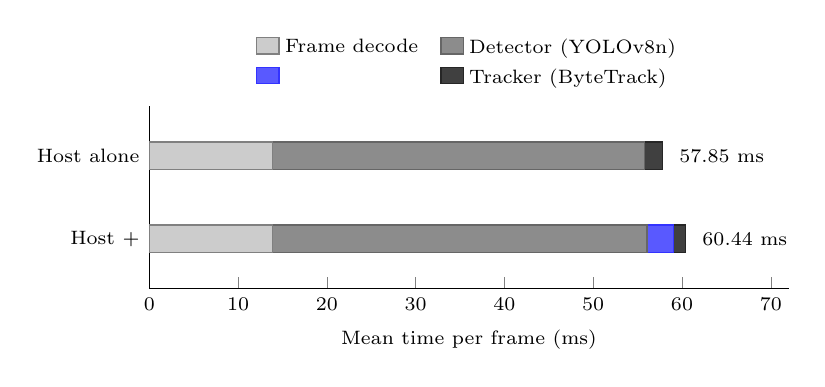
\begin{tikzpicture}
\begin{axis}[
  xbar stacked,
  /pgf/bar width=10pt,
  width=0.8\columnwidth,
  height=3.9cm,
  xmin=0, xmax=72,
  clip=false,
  ymin=-0.6, ymax=1.6,
  ytick={0,1},
  yticklabels={Host + \scl{}, Host alone},
  xlabel={Mean time per frame (ms)},
  axis x line*=bottom,
  axis y line*=left,
  tick label style={font=\scriptsize},
  label style={font=\scriptsize},
  legend style={at={(0.5,1.04)}, anchor=south, legend columns=2,
    font=\scriptsize, draw=none, /tikz/every even column/.append style={column sep=6pt}},
  legend cell align=left,
]
\addplot[fill=black!20, draw=black!50] coordinates {(13.88,1) (13.88,0)};
\addplot[fill=black!45, draw=black!60] coordinates {(41.91,1) (42.17,0)};
\addplot[fill=blue!65, draw=blue!80] coordinates {(0,1) (2.95,0)};
\addplot[fill=black!75, draw=black!85] coordinates {(2.04,1) (1.43,0)};
\legend{Frame decode, Detector (YOLOv8n), \scl{}, Tracker (ByteTrack)}
\node[anchor=west, font=\scriptsize] at (axis cs:58.6,1) {57.85 ms};
\node[anchor=west, font=\scriptsize] at (axis cs:61.2,0) {60.44 ms};
\end{axis}
\end{tikzpicture}

\caption{Mean per-frame time by stage for the host pipeline alone and with
\scl{} (4-vCPU Intel Xeon, no GPU). The labels give the measured
end-to-end time.}
\label{fig:runtime}
\end{figure}
